% !TEX root=../../report.tex

\Section{Nichtfunktionale Anforderungen}

Einige Anforderungen lassen sich nicht aus Anwendungsfällen ableiten. Sie beinhalten keine zusätzlichen Funktionen für die Anwendung, sondern beschäftigen sich mit Sicherheits- und Performanceaspekten, sowie der Benutzerfreundlichkeit des Systems. Da diese auf keinen Fall zu vernachlässigen sind, werden sie auch besprochen und dokumentiert.

\subsubsection{Sicherheit}

Ein sehr wichtiger Aspekt einer Anwendung ist die Sicherheit. Es soll beispielsweise verhindert werden, dass Benutzer Änderungen durchführen können, zu welchen sie nicht berechtigt sind. Weiterhin dürfen sie auch nur Informationen erhalten, die für sie bestimmt sind.

Der EventManager nutzt ein \enquote{Claims-based Security System}. Ein \enquote{Claim} ist eine Information, die über ihren Besitzer bekannt ist, und als Tatsache betrachtet wird (siehe \myref{jwt}). Die Claims werden durch die Anmeldung abgefragt und bis zum Abmelden gespeichert. So kann vor der Ausführung von Aktionen überprüft werden, ob der angemeldete Benutzer die nötigen Berechtigungen dafür besitzt. Ist dies nicht der Fall, wird eine entsprechende Fehlermeldung ausgegeben.

\subsubsection{Benutzerfreundlichkeit}

Die Nutzeroberfläche der Webseite wird an das Material Design von Google angelehnt. Die Oberflächenentwürfe werden im Team besprochen, um sicherzustellen, dass die Seite möglichst angenehm und effizient genutzt werden kann. Es fällt jedoch schnell auf, dass mit Erfahrungswerten und Vermutungen argumentiert wird und keine fundierten Designaspekte vorgebracht werden.

\begin{figure}[h]
\centering
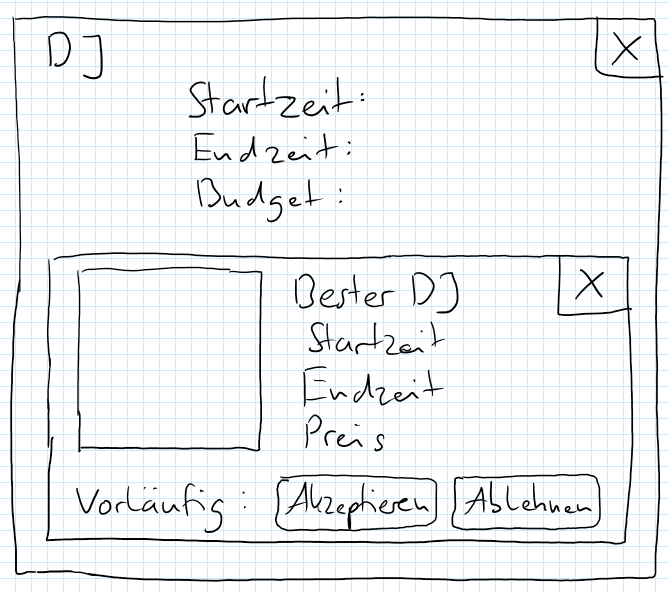
\includegraphics[width=.5\textwidth]{res/images/ServiceSlot.png}
\caption{Oberflächenentwurf eines Dienstleistungsslots}
\label{ss}
\end{figure}

Die \myautoref{ss} zeigt den Oberflächenentwurf eines Serviceslots. Der Entwurf konzentriert sich darauf, den Anforderungen an einen solchen Slot zu genügen.

Die Kategorie, welcher der Slot zugeordnet ist, steht an erster Stelle, nachfolgend die Rahmenbedingungen. Ist dem Slot ein Dienstleister zugeordnet, werden dessen Informationen mit angezeigt. Dies sind der aktuelle Vereinbarungsstatus, die Start- und Endzeit, sowie das Budget.



% Da Anforderungen festgelegt wurden, nach denen sowohl das Löschen der Vereinbahrung, als auch des eigentlichen Slots vorgesehen werden soll, werden Buttons dafür angebracht. Sie werden gewohnt positioniert, nämlich rechts oben. Außerdem werden noch zwei weiter Buttons zum Akzeptieren und Ablehnen einer Vereinbahrung angebracht, um die Arbeit mit den Serviceslots zu erleichtern.

Die Funktionen zum Löschen, Bearbeiten und Suchen von Dienstleistern werden erst angeboten, wenn man auf den Slot klickt und damit auf die nächste Seite navigiert.
